%!Mode:: "Tex:UTF-8"
\chapter{引言}\label{chap:introduction}


\section{复杂网络的研究背景及意义}

随着人类的进步和社会的发展, 人与人之间、人与自然界之间以及自然与自然之间形成各种千姿百态、形形色色的复杂网络系统, 例如社交关系系统、电力系统、航空系统、万维网、食物链、疾病传播系统、蛋白质相互作用系统等等. 人们为了研究这些网络系统的特征和性质, 抛开系统的物理和社会含义, 把系统中互异的元素称之为节点(node), 把元素之间的关系用连边(edge) 来表示, 于是物理网络系统都可以抽象为由节点和连边组成的复杂网络模型. 例如, 在社会关系系统中, 可以把每一个人看做网络的节点, 如果两个人之间相互认识, 那么就用连边表示; 在航空系统网络中, 我们可以把各个城市看做网络的节点, 若城市之间存在航线, 就用连边来表示. 由此可见, 任何一个复杂的网络系统都可以将其抽象成为具有节点和连边的网络结构. 这种从具体网络模型上升到抽象网络模型的思想给研究者探索网络内部结构的复杂性提供了一种新思路.

这种将真实网络中的实体与实体之间的关联抽象化成为节点和连边所组成的复杂网络的思想是源于$18$世纪$30$年代著名数学家Eular论证哥七桥问题. Eular首次将真实存在的物理关系抽象为节点与连边, 从而开创图论学科, 使网络研究最终独立成为一门学科. 从此掀起了科学家们对网络科学理论的研究热潮. 早些年, 研究者们研究的网络模型都是具有某种特殊结构的网络, 也就是说网络中的节点与节点关系遵循一定的规律, 这种网络称为规则网络. 主要的规则网络有完全连接网络、最近邻连接网络、星形网络、Lattice网络、Layers网络等. 但是对于大规模网络而言, 它的复杂程度并不是都能采用规则网络来表征.

1960年前后, 两位杰出的数学大师Erdös与Rényi创立了著名的随机图理论, 从而为随机网络(ER Network)的发展奠定了理论基础. 随机网络与规则网络最大的不同点在于网络节点间的关系不再是确定的, 而是以一定的概率随机连接的. 由于复杂网络节点之间的关系是受到随机变量的控制, 从而使得网络耦合拓扑空间变得更为复杂, 并且在数学性质上与规则网络也存在质的不同, 很多规则网络的性质在随机网络中不在成立. Erdös和Rényi两人在研究时发现, 随机网络的重要特征和性质都是随着节点数量的扩大而突出出现的.

\begin{figure}[htb]
\begin{minipage}[t]{0.48\linewidth}
\centering
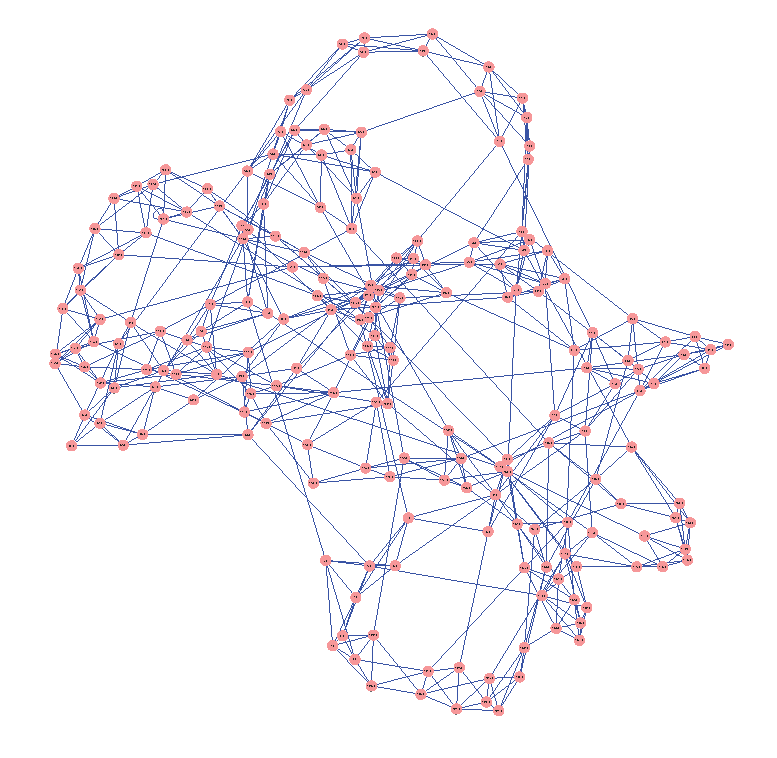
\includegraphics[width=2.5in]{introduction/wattsstrogatz.eps}
\caption{小世界网络.}\label{smallworld}
\end{minipage}~~
\begin{minipage}[t]{0.48\linewidth}
\centering
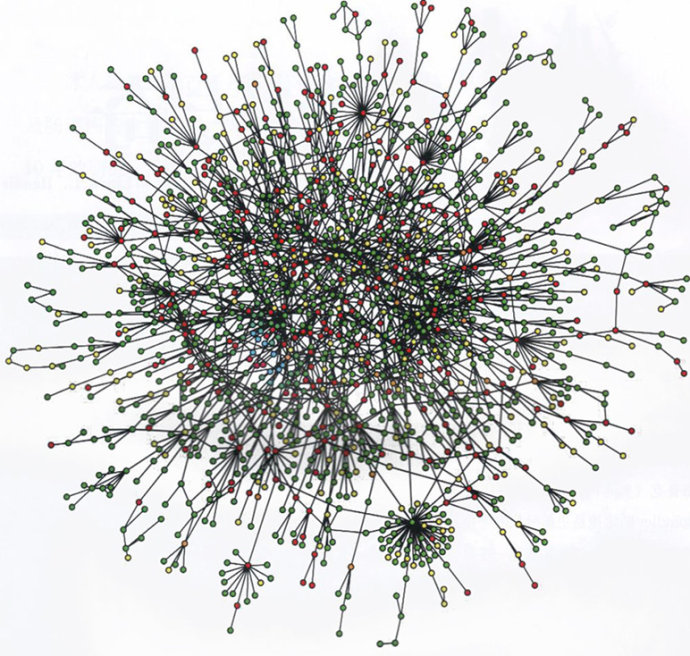
\includegraphics[width=2.5in]{introduction/scale.png}
\caption{无标度网络.}\label{scalefree}
\end{minipage}
\end{figure}

20世纪末, 科学家们发现, 很多网络都具有高度的集群性、不均衡的度分布以及中心节点结构. 这类结构的网络恰好是介于规则网络和随机网络之间, 但是它的统计特征与规则网络和随机网络截然不同. 国际上出现两项具有里程碑意义工作: Watts 和Strogatz在1998年定义了一种新型网络—小世界网络\upcite{2}(如图 \ref{smallworld}). 小世界网络介于规则网络和随机网络之间, 它是在规则网络的基础上以一定的概率断开连边后在重新随机连接其他的节点所形成的网络. 当切断连边的概率取$0$、$1$ 两个极端值的时候, 此时就变成规则网络和随机网络(如\autoref{SWN}). 生活中的很多网络都表现出小世界特性, 例如蛋白质分子相互作用网、手机通讯网络、科学引文网以及社会关系网等. 小世界网络的提出, 进一步证实了“六度分离”假说.

%在小世界网络出现之前, 人们认为网络分为完全规则网和完全随机网, 这两类网络具有各自的特征. 规则网络具有较大的特征路径长度, 聚类系数也较大, 而随机网络具有较小的特征路径长度, 但是聚类系数较小. 但现实中的网络如电网、交通网络、脑神经网络、社交网络、食物链等都表现出小世界特性, 即具有较高的聚类度和较小的特征路径长度. 也就是说小世界网络中大部份的节点彼此并不相连, 但绝大部份节点之间经过少数几步就可到达.
\begin{figure}[htb]
  \center
  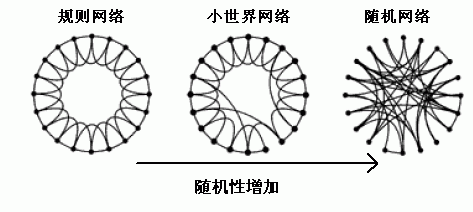
\includegraphics[width=3.3in]{introduction/smallnetwork.png}\\
  \caption{规则网络、小世界网络、随机网络之间的关系.}\label{SWN}
\end{figure}

一年后, Barabási等人于1999年在《科学》杂志上出了另外一种非均匀的网络模型——无标度网络\upcite{0}(如\autoref{scalefree}). 这类网络不仅拥有较大的聚类特性和较小的平均路径长度, 而且节点的度服从幂律分布. 许多复杂网络系统, 例如因特网路由关系网, 人力资源关系网等, 其网络中的大多数节点都是与某些特殊的节点有关联, 即网络中存在个别具有主要控制能力的节点. 这种网络节点间关系的不均匀性称为无标度网络的无标度性, 这种不均匀性是网络内在的一种性质.
复杂网络的“小世界”与“无标度”等统计特性的发现, 不仅丰富了网络内部结构的拓扑形式, 更进一步推动了研究者对复杂网络结构不断探索的热潮, 同时也加快了复杂网络理论在各个学科的研究进程\upcite{4,5,6,7,8,9,10}.

进入21世纪后, 小世界效应和无标度特性的提出使得复杂网络的理论研究踏上新台阶 , 并形成多学科交叉的理论成果. 近年来, 众多理论模型和分析方法如雨后春笋般涌现, 并且尝试利用复杂网络理论成果来解决各领域的实际问题. 目前主要研究工作分为: 一是研究网络内部耦合结构的变化以及统计性质, 例如网络系统的平均路径长度、聚集系数、度及度分布、谱性质、介数、小世界效应、无标度特性等特征; 二是研究复杂网络动力学行为, 包括鲁棒性、稳定性、一致性、以及同步问题等; 三是复杂网络在各个领域的应用, 包括生物医学、保密通信、图像处理、交通运输等领域\upcite{15,16,17}.


\section{复杂网络同步控制及其研究现状}
同步(synchronization)指的是两个或者两个以上性质相同或相似的动力系统通过系统节点之间的相互影响使得各个节点的动力学行为随着时间演变慢慢地趋于同一步调. 复杂网络的同步是一种群集行为. 自然界中同步现象数不胜数, 其中两个最为经典的同步现象是: 1665年, 荷兰物理学家、数学家惠更斯发现自家墙上的两个挂钟不论钟摆开始时如何摆动, 一段时间后, 两个摆钟的摆动频率完全相同, 摆动的方向恰好相反; 1680年, 荷兰旅行家肯普弗在旅行时注意到一个奇特的现象: 停留树枝上的萤火虫闪光的频率非常有规律, 几乎都是同时闪或者不闪. 除此之外, 生活中还存在各式各样的同步现象, 例如鱼群朝同一方向游动, 大雁群的一致飞行, 演唱会观众的拍手声等等.

1990年Pecora和Carroll\upcite{10}发现了一类混沌系统的同步现象, 由此开启了同步理论的研究新篇章. 目前已经出现了各种不同形式的同步模式:
有限时间同步\upcite{finitetimesyn}、固定时间同步\upcite{fixsyn}、完全同步\upcite{abssyn}、 簇同步\upcite{clusyn}、位相同步\upcite{phasyn}、指数同步\upcite{23}. 其中, 完全同步指的是只需要当时间趋于无穷时, 网络所有的节点之间的误差趋于零, 它是同步模式中最普遍的一种. 而指数同步是指误差以指数形式趋于零, 它是比完全同步具有更快同步速度的同步模式. 本文仅讨论这两种同步模式.

在近十多年里, 人们对各种复杂网络拓扑模型的同步问题进行了广泛地研究并积累了大量的研究成果\upcite{Karimi5,Multi6,Lu7,Liu8,Karimi10,Lu9,Turci11,Jin12,Turci13}. %2014 年Wang和Tang等人\upcite{p30,p31}对近十年来复杂网络的研究成果进行了概括总结, 并指出未来复杂网络研究的挑战.
但大多数的研究成果都是基于理想的假设: 网络所处的环境是保持不变的, 即网络的耦合结构、耦合强度是固定的, 且网络节点间的通讯不会受到其他外在因素的干扰. 然而, 在实际问题中, 这个假定很难被认为是合理的. 事实上, 在现实应用中, 网络系统的节点状态、耦合结构和耦合强度不可避免地遭受来自外部随机因素的干扰.
例如电力输送网会受到地震、火灾、雷击、输变电系统短路等不可预知因素的影响; 保密通讯会受到黑客的攻击等等.
因此考虑随机环境下的网络同步更加具有实际意义.
最近几年, 研究者们开始重视随机环境下复杂网络同步问题, 并且现在成为了一个较为活跃的研究方向. 随机环境下复杂网络同步问题研究的主题包括: 一是运用连续时间马尔可夫链来模拟耦合结构受随机环境影响而切换的变化过程\upcite{Li15,p10Markovian,p11Markovian,mm19,M20,M21,M22,M23,M24,M25,M17}; 二是引入随机变量来刻画耦合强度的随机性以及随机发生的耦合关系\upcite{X18,M19,randomcoupling1}; 三是通过布朗运动来模拟随机噪声对网络节点自身以及节点之间信号传输过程的干扰\upcite{Eventmultiagentnoises,p29,p30,p31,p32}. 尽管随机环境下复杂网络同步问题的研究取得较大的进展, 但还有许多问题亟待解决.
例如, 节点间状态信息的传输并非是简单的线性可观测形式, 而是通过非线性映射后的形式; 信息传输的有限速度和带宽引起网络节点自身动力学时滞的问题, 马尔可夫链转移率获取困难而引起的部分未知转移率的切换拓扑同步问题, 等等. 这些问题的解决能够更进一步完善复杂网络同步理论.

在现实生活中, 网络很难依靠自身节点之间的拓扑关联实现同步(自然同步)\upcite{phasyn,natsyn}. 这是由于网络内部节点庞大, 节点间的关联较为稀疏, 并且网络节点的关系会遭受到外部随机因素的干扰. 因此, 需要对网络施加外力, 即通过设置控制器来促使网络实现的同步.
目前, 很多控制策略被提出. 比较经典而且经济的控制策略是牵制控制\upcite{pin1,pin2,pin3}. 它只需要控制系统中极少数重要的节点, 然后通过节点的耦合关系将控制输入信号传送到其他的节点, 从而使得整个网络在控制节点的带领下达到同步状态. 相对于全局控制, 牵制控制具有可操作性强且节省控制成本的优势.
然而, 很多全局控制或者牵制控制的同步成果都是在连续通信模式下建立的, 这使得系统连续不断地更新自身信息状态和控制输入信号, 并且实时地向邻居节点发送当前状态信息. 显然, 这种模式会导致不必要的带宽和能源消耗, 加大了网络的通讯负荷, 并且降低了网络抗干扰能力.

随后, 研究者们提出了数据采样机制来降低节点间的通讯以及控制输入的更新频率, 数据采样机制主要有周期采样\upcite{period}以及事件激发采样. 根据周期选取的不同, 周期采样又分为固定周期采样、时变周期采样、以及随机周期采样. 相对于连续通信模式, 周期采样以可变频率进行采样并更新节点状态和控制项, 一定程度上节省了控制成本, 并且减少了节点间的通讯频率. 尽管周期采样模式能够减小能量的消耗和降低网络的通讯负荷, 但是该通讯模式对周期的选择较为敏感, 若周期过短会导致较大的计算负荷, 若周期过长会导致同步速度较慢. 除此之外, 网络不能够根据各个节点的状态自动地改变采样数据的频率. 不同于周期采样, 事件激发采样机制能够根据网络自身节点间的关系以及节点与同步目标之间的误差来决定采样时刻, 即系统能够根据自身的运行状况自适应地调整采样时间点, 事件激发采样机制正好弥补了周期采样在周期选择上的缺陷. 事件激发采样控制策略被广泛应用于多主体系统一致性控制问题\upcite{Eventmultiagentnoises,eventmult2,eventmult3,eventmult4,eventmult5,eventmult6,eventmult7,eventmult8,eventmult9}, 最近有研究者开始关注事件激发采样控制策略在复杂网络同步问题的研究, 并取得了一些进展性工作\upcite{eventsyn1,eventsyn2,eventsyn3,eventsyn4,eventsyn5,eventsyn6,eventsyn7}. 事件激发采样模式的主要思想是: 当系统节点与同步目标之间的偏差大于给定的阈值时, 此时事件被触发, 节点就更新自身的状态和控制项, 并向邻居节点传递信息. 换句话说, 网络节点的信息更新和信号的传输只发生在事件激发时刻. 事件激发采样控制模式最大的特点是网络根据节点自身的状态按照需要进行更新和传递数据信号, 从而能够极大减少通信的频率, 节省能量. 正如K. {\AA}ström\upcite{eventsyn8} 和B. Wang\upcite{eventsyn9}等人证实, 事件激发采样控制策略比周期采样策略表现出更好性能.

事件激发采样策略的核心在于根据网络节点间的关系定义激发规则. 按照激发时刻是否一致可以分为集中式激发规则\upcite{Eventmultiagentnoises}和分散式激发规则\upcite{eventmult3}; 按照监控时间是否连续可以分为连续监控激发规则\upcite{eventsyn5}和离散监控激发规则\upcite{eventsyn7}. 连续监控激发规则不仅依赖于节点及其邻居最新激发时刻状态信息, 而且依赖于节点当前的状态信息, 即需要对节点的状态进行实时的监控. 而离散监控激发规则只需根据最新激发时刻的状态信息对下一次激发时刻进行预测, 在下一次激发到来之前, 节点的状态不需要进行监控. 这两种激发规则各有利弊, 连续监控激发规则花费较大的监控成本, 但是激发频率较低, 因而有效地降低了网络节点间的通讯负荷, 更有利于维持网络的稳定性; 而离散监控激发规则监控成本较低, 但会增加激发频率, 加大通讯负荷. 在实际应用中一般根据监控成本和通讯负荷来衡量运用那种激发规则. 集中式激发规则要求所有节点的激发时刻一致, 即根据网络节点的信息状态对每个节点定义统一的激发规则. 而分散式激发规则每个节点根据自身状态和邻居最新的更新信息定义自己的事件触发规则. 相比较而言, 集中式采样策略具有更低的计算负荷, 并且能更快地促使系统达到同步, 但激发频率比分散式采样策略要高.

目前, 利用事件激发采样策略研究复杂网络问题还处于起步阶段, 主要集中在以下几个方面: 一是通过有限时间事件激发研究带马氏链的非线性系统鲁棒性的问题\upcite{eventnonlinear}; 二是利用事件激发通讯协议研究带马尔可夫跳网络的状态估计问题\upcite{eventMarkov4, eventdelay3}; 三是设计事件激发通讯策略研究多主体系统一致性问题\upcite{consensus1,consensus2}; 四是基于事件激发采样控制策略研究一般马氏切换拓扑复杂网络的同步问题\upcite{eventMarkov3,eventMarkov0,eventMarkov2}; 五是采用事件激发采样协议研究转移率未知的马氏跳复杂网络的控制问题\upcite{eventdelay1,eventunknown}. 尽管事件激发采样技术在网络研究方面已有相关的理论成果, 但为数不多. 特别是在复杂网络的同步问题上, 一方面, Liu、Shao、Wang等人\upcite{eventMarkov3,eventMarkov0,eventMarkov2}所考虑的都是简单的线性耦合系统, 同时也未考虑到耦合关系随机中断、耦合强度随机变化的情况, 除此之外, 他们也没有在离散监控的情形下设计事件激发采样策略. 另一方面, 对于转移率未知的问题, Senan\upcite{eventdelay1}讨论了带混合时滞的转移率未知的带马尔可夫跳神经网络的同步问题, Li\upcite{eventunknown}给出了转移率未知的马氏跳网络随机稳定性的充分条件, 并给出了事件激发的下界, 证实了Zeno 现象不会发生. 然而, 对于部分转移率未知、动态同步目标以及时滞共存的复杂网络同步问题并未发现相关成果, 此外对于节点状态信息在传输过程中受到噪声干扰的模型也未见有研究者们利用事件激发采样技术来给出同步判据. 这些网络模型同步问题的解决, 能够更一步地完善事件激发采样策略下复杂网卡控制同步问题的理论. 本文将逐一讨论运用事件激发采样控制去研究这类带有随机因素影响的复杂网络同步问题.

%
%例如, Li等人\upcite{eventsyn1}应用事件激发策略与间歇通讯策略相结合研究了动态复杂网络的同步问题; Chen 等人\upcite{eventsyn2}分别设置连续监控激发规则和离散监控激发规则研究线性耦合复杂网络的同步问题; Lu等人\upcite{eventsyn7} 通过事件激发策略与牵制控制方法得出了带马尔科夫切换线性耦合复杂网络的同步判据; Lang等人\upcite{eventsyn5}基于事件触发策略研究了带迟滞的神经网络的同步问题; Guinaldo 等人\upcite{packetloss} 通过事件触发策略研究了带迟滞和数据包丢失的复杂网络的同步问题. 尽管事件激发控制策略在同步问题上得到了较好的应用, 但仍然有一些问题有待解决. 上述成果很少有考虑到随机环境对系统的影响. 特别是噪声对信号传输过程的干扰以及控制器偶然失败的情况. 除此之外, 马尔可夫调制的耦合结构在状态切换时的转移概率并非完全已知, 并且非线性的耦合方式更是具有挑战性. 本文将讨论运用事件激发控制去研究这类复杂网络的同步问题.


\section{本文的主要工作及创新点}

本文主要利用基于事件激发采样策略的离散通讯模式研究几类带有马尔可夫切换的复杂网络同步问题. 通过设定合适的事件激发规则, 基于Lyapunov稳定性理论、矩阵理论、随机过程理论等知识推导出几类马尔可夫切换网络的同步判据, 并给出数值模拟例子说明推导的同步条件是有效性的.

本学位论文工作分为以下六个部分:

第一章介绍复杂网络及其同步的研究背景和意义, 简单概述和分析国内外有关复杂网络同步研究的现状, 并介绍复杂网络常用控制方法以及基于事件激发控制策略的优点, 最后简要叙述本文工作及创新点.

第二章给出复杂网络的理论和模型, 介绍随机过程理论的基础知识, 最后给出复杂网络同步的数学定义、证明主要结论所有的引理、及本文所用的记号.

第三章对非线性随机发生耦合的复杂网络同步问题进行了研究. 网络模型是在卢文联2015年研究的一篇文章\upcite{eventsyn2}基础上进行改进, 模型不仅包含了马氏切换和非线性耦合, 而且也考虑了网络节点间的耦合关系和耦合强度受到随机因素影响的情形, 即随机发生的耦合和随机耦合强度. 基于分散式事件激发控制策略下, 分别给出连续监控形式的同步误差上界(CRS) 和指数函数上界(CRE) 激发规则以及离散监控情形下的同步误差上界(DRS)和指数函数上界(DRE)激发规则. 利用稳定性理论、随机过程理论、以及矩阵分析理论推导出同步的充分条件. 最后, 对于四种不同激发策略, 分别比较其优缺点和适用场景. 并给出一个数值仿真来验证本节结论的有效性.

第四章基于集中式事件激发策略研究了部分转移率未知时滞的复杂网络同步问题. 本章在第三章的基础上进行拓展, 在马氏切换拓扑的基础上, 对部分转移率未知以及节点自身动力学存在时滞的网络进行研究. 基于集中式事件激发策略, 设计随机发生的控制器来促使网络达到同步. 在稳定性理论、随机过程理论、以及矩阵分析理论下证实给出的同步判据是充分有效的. 同时, 也给出了几个一般模型下的推论. 最后给出事件激发间隔的下界, 从而证实Zeno现象不会发生. 数值仿真揭示理论结果的有效性. 本章的主要结果已发表在Applied Mathematics and Computation杂志.

%由于网络带宽有限, 信号的传输可能会发生延迟, 因此考虑迟滞的复杂网络模型更加符合实际.
%除了系统上的改进外, 在目标节点的选择上也做了改进. 前两章主要考虑的是已知同步目标, 也就是说网络同步目标$s(t)$是根据孤立节点动力学$s(t)=\dot{f}(s(t))$确定的, 这在有些场合并不适合. 例如, 在讨论会上我们并没有提前讨论的结果, 讨论的结果是通过讨论者的观点不断影响他人, 最后大家形成一致的意见或者得出同一的解决方案. 因此研究动态同步目标也是有必要的. 另外, 本节还给出了事件激发区间的下界, 从而避免了Zeno现象. 最后

第五章研究部分转移概率未知带噪声干扰的复杂网络同步问题. 通过引进布朗运动模拟网络节点间信号传输过程中噪声的影响, 分别在集中式和分散式事件激发策略下, 构造马氏调制的线性控制器. 然后利用伊藤公式、Lyapunov 稳定性定理等知识, 给出部分转移概率未知且带随机扰动马尔可夫网络的同步判据. 最后通过实验仿真证实定理给出的判定条件的有效性.

%前两章主要分析了非线性和时滞模型, 考虑马尔可夫链的转移率是部分未知以及带噪声扰动的情形. 因为耦合关系的切换有时候并不完全知道切换的概率, 同时网络节点之间的信息传输会受到噪声的干扰, 从而导致网络的不稳定性. 所以本节主要研究部分未知转移率且带有噪声的马尔可夫网络.

第六章针对本文的工作进行简要概括和总结, 以及对以后研究方向进行展望.

本文的主要创新点如下:
\begin{itemize}\setlength{\itemsep}{0cm}
  \item
  %线性耦合结构的复杂网络同步问题已经得到广泛研究, 并且具有较丰富的理论结果. 非线性耦合尽管有一些成果, 但也都是建立在连续采样或者周期采样的模式下, 这在一定程度上会加大网络节点间的通讯负荷.
  目前基于事件激发策略的控制方法研究非线性耦合关系马氏切换网络的理论结果还未有人提及. 本文在线性基础上, 研究了随机发生的非线性耦合、随机耦合强度以及事件激发控制模式共存的网络模型同步问题;
  \item 在网络耦合关系随机性方面, 本文不仅以马氏切换模拟随机切换拓扑, 还考虑耦合关系在切换过程中的转移率是部分未知. 除此之外, 网络节点存时滞的情况也加入到模型中, 同时引进动态的同步目标. 设置合适的事件激发策略控制网络达到同步;
  \item 针对部分转移概率未知时滞的网络模型, 给出事件激发区间的下界, 证实了Zeno现象不会发生;
  \item 噪声是一项不可避免的随机因素, 而噪声一般对网络节点自身和网络节点间通讯都会造成影响. 相对于网络节点自身, 通讯干扰对网络稳定性影响更大. 很多研究者往往只考虑了节点自身动力学行为受到噪声扰动, 而本文在离散通讯模式下加入布朗运动模拟节点间的信号传输过程中受到噪声扰动.
\end{itemize}


